\documentclass[onecolumn,12pt]{article}

%----Wgranie packages----------
\setlength{\voffset}{-0.55in}
\setlength{\headsep}{3pt}

\usepackage{hyperref}
\hypersetup{
    colorlinks=false, %set true if you want colored link
    linktoc=all,     %set to all if you want both sections and subsections linked
}

\usepackage[polish]{babel}
\usepackage{algorithm,algorithmic,lipsum}
\usepackage[utf8]{inputenc}
\usepackage{url}
\usepackage{anyfontsize}
\usepackage{multirow}
\usepackage{subfigure}
\usepackage{tabularx}
\usepackage{ragged2e}
\usepackage{booktabs}
\usepackage{multirow}
\usepackage{grffile}
\usepackage{indentfirst}
\usepackage{caption}
\usepackage{listings}
\usepackage{lipsum}
\usepackage{enumitem}
%\usepackage{xcolor}
%\usepackage{hyperref}
\usepackage{catchfilebetweentags}
\usepackage[smartEllipses]{markdown}
\usepackage[ruled,linesnumbered,lined]{algorithm2e}
\usepackage[bookmarks=false]{hyperref}
\usepackage{mathtools}
\DeclarePairedDelimiter\ceil{\lceil}{\rceil}
\DeclarePairedDelimiter\floor{\lfloor}{\rfloor}

\hypersetup{colorlinks,
    linkcolor=blue,
    citecolor=blue,
    urlcolor=blue}

\usepackage[svgnames]{xcolor}
\usepackage{inconsolata}
\usepackage{fontawesome}

\usepackage{csquotes}
\DeclareQuoteStyle[quotes]{polish}
    {\quotedblbase}
    {\textquotedblright}
    [0.05em]
    {\quotesinglbase}
    {\fixligatures\textquoteright}
\DeclareQuoteAlias[quotes]{polish}{polish}

\usepackage[nottoc]{tocbibind}
\usepackage[
style=numeric,
sorting=nyt,
isbn=false,
doi=true,
url=true,
backref=false,
backrefstyle=none,
maxnames=10,
giveninits=true,
abbreviate=true,
defernumbers=false,
backend=biber]{biblatex}

\lstset{
        %language=Python,  %%  PHP,  C,  Java,  etc.
        basicstyle=\ttfamily\footnotesize,
        backgroundcolor=\color{gray!5},
        commentstyle=\it\color{Green},
        keywordstyle=\color{Red},
        stringstyle=\color{Blue},
        numberstyle=\tiny\color{Black},        
        %  morekeywords={TestKeyword},
        %  mathescape=true,
        escapeinside=`',
        frame=single,  %shadowbox,  
        tabsize=2,
        rulecolor=\color{black!30},
        title=\lstname,
        breaklines=true,
        breakatwhitespace=true,
        framextopmargin=2pt,
        framexbottommargin=2pt,
        extendedchars=false,
        captionpos=b,
        abovecaptionskip=5pt,
        keepspaces=true,                        
        numbers=left,                                        
        numbersep=5pt,                                    
        showspaces=false,                                
        showstringspaces=false,
        showtabs=false,
        tabsize=2
    }

\definecolor{graytext}{gray}{0.6}

\lstdefinestyle{PostgreSQL}{
    literate={ą}{{\k a}}1
    		 {Ą}{{\k A}}1
             {ż}{{\. z}}1
             {Ż}{{\. Z}}1
             {ź}{{\' z}}1
             {Ź}{{\' Z}}1
             {ć}{{\' c}}1
             {Ć}{{\' C}}1
             {ę}{{\k e}}1
             {Ę}{{\k E}}1
             {ó}{{\' o}}1
             {Ó}{{\' O}}1
             {ń}{{\' n}}1
             {Ń}{{\' N}}1
             {ś}{{\' s}}1
             {Ś}{{\' S}}1
             {ł}{{\l}}1
             {Ł}{{\L}}1,
    keywordstyle=\textbf,
}

\SetAlgorithmName{\LangAlgorithm}{\LangAlgorithmRef}{\LangListOfAlgorithms}
\newcommand{\listofalgorithmes}{\tocfile{\listalgorithmcfname}{loa}}

\renewcommand{\lstlistingname}{\LangListing}
\renewcommand\lstlistlistingname{\LangListOfListings}

\renewcommand{\lstlistoflistings}{\begingroup
\tocfile{\lstlistlistingname}{lol}
\endgroup}

\begin{document}
% ----------Strona tytułowa------------
\title{Eksploracja Danych - Projekt\\
Analiza czynników wpływających na występowanie chorób}
\author{Gabriela Bocheńska, Aleksandra Stachniak, Gabriela Piwar}
\date{\today}
\maketitle

% ----------Spis treści------------
\tableofcontents
\thispagestyle{empty}
\newpage

% ----------Raport------------
\section{Wprowadzenie}

---- WERSJA WIP ---- 

Choroby cywilizacyjne są głównymi przyczynami przedwczesnej śmiertelności i chronicznej niepełnosprawności na całym świecie. Według danych ze Stanów Zjednoczonych [data needed] te schorzenia dotykają miliony Amerykanów, stanowiąc znaczące obciążenie dla systemu opieki zdrowotnej. Do najczęsztyszch możemy zaliczyć cukrzycę, nadciśnienie i udar mózgu.

Cukrzyca to grupa zaburzeń metabolicznych charakteryzujących się wysokim poziomem glukozy we krwi, wynikającym z problemów z produkcją lub działaniem insuliny – hormonu produkowanego przez trzustkę. Istnieją dwa główne typy cukrzycy: typ 1 - wrodzony, gdzie organizm nie produkuje insuliny oraz typ 2 - nabyty, który jest często spowodowany przez niezdrowy tryb życia. Ponieważ
drugi typ jest ściśle związany z nadwagą, brakiem aktywności fizycznej, niezdrową dietą oraz innymi powiązanymi czynnikami, istnieje ogólne ryzyko, że może on dotknąć niemal każdego, kto nie stosuje się do zaleceń zdrowotnych.

Nadciśnienie tętnicze, często nazywane "cichym zabójcą", polega na nieprawidłowo wysokim ciśnieniu krwi w tętnicach, co może prowadzić do uszkodzenia wielu narządów, w tym serca, nerek, mózgu i oczu. Nadciśnienie często rozwija się przez wiele lat bez widocznych objawów, ale może być spowodowane czynnikami takimi jak otyłość, brak aktywności fizycznej, nadmierne spożycie soli, palenie tytoniu oraz czynniki genetyczne. Wczesne wykrycie i leczenie, głównie poprzez zmiany stylu życia i farmakoterapię, są kluczowe dla zapobiegania długoterminowym komplikacjom.

Udar mózgu występuje, gdy przepływ krwi do części mózgu zostaje nagle przerwany, co może być spowodowane zatorem (udar niedokrwienny) lub pęknięciem naczynia krwionośnego (udar krwotoczny). Objawy mogą obejmować nagłe osłabienie, trudności w mówieniu, zrozumieniu mowy, widzeniu, utratę równowagi lub nagłe, silne bóle głowy. Czynniki ryzyka udaru są podobne do tych dla nadciśnienia i cukrzycy, obejmujące niezdrową dietę i brak aktywności fizycznej.

\newpage

\section{Cel projektu}

Celem niniejszego projektu jest zidentyfikowanie populacji osób narażonych na podwyższone ryzyko
wystąpienia przewlekłych chorób takich jak cukrzyca, nadciśnienie tętnicze oraz udar mózgu. Analiza ma na celu wykazanie wpływ stylu życia na rozwój i progresję różnych chorób za pomocą nowoczesnych technik wczesnego wykrywania patologii, pozwalających do szybszej diagnozy wymienionych schorzeń.

Założenia projektu obejmują wnikliwą analizę danych, polegającą na przetworzeniu i interpretacji zawartych informacji w zbiorze. Na jej podstawie w projekcie stworzono kilka modeli predykcyjny, które za zadanie miały identyfikację osób znajdujących się w grupie ryzyka z dużą dokładnością.
        
\section{Zbiór Danych}

\subsection{Opis zbiorów}
Zbiór danych wykorzystany w projekcie pochodzi z witryny Kaggle (Diabetes, Hypertension and Stroke Prediction) i jest wynikiem połączenia trzech różnych zestawów danych dotyczących zdrowia, zawierających odpowiednio wskaźniki cukrzycy, niewydolności serca oraz udaru. Każdy zbiór został wcześniej poddany obróbce w celu wyrównania liczebności klas. W zbiorze znalazły się w nim:

\begin{enumerate}
  \item Pierwszy zestaw danych również pochodzi z Kaggle (Diabetes Health Indicators Dataset). Zawiera 18 cech zdrowotnych związanych z cukrzycą. Do najważniejszych możemy zaliczyć fizyczne cechy takie jak poziom glukozy we krwi, BMI, wiek oraz cechy związane z trybem życia, takie jak ilość spożywanych warzyw i owoców w ciągu dnia, ilość wypijanego alkoholu czy liczba dni kiedy osoba stwierdza u siebie złe samopoczucie. 
  
  \item Drugi zestaw danych, używany w analizie niewydolności serca, pochodzi z witryny smellydatascience.com. Obejmuje on 14 cech,  głównie są to cechy fizyczne pacjenta np. wiek i płeć. Inne zmienne jak ciśnienie krwi, cholesterol oraz wyniki badania EKG są ściśle związane z przeprowadzeniem konkretnych badań. Otrzymane dane ściśle nie opisują trybu życia pacjenta, jednak dają infromację o jego skutkach.
  
  \item Trzeci i ostatni zestaw danych, dostępny także na Kaggle (Stroke Prediction Dataset). Zawiera on podobne wskaźniki zdrowotne jak w pierszym zbiorze, skupiając się na trybie życia pacjenta, takie jak stan cywilny, rodzaj miejsca zamieszkania ale też czy wystąpiły inne choroby u pacjenta związane z układem krążenia. 
\end{enumerate}

\subsection{Oczyszczenie danych}
W procesie oczyszczania danych zastosowano kilka zaawansowanych technik mających na celu poprawę jakości i spójności zbiorów danych. Pierwszym krokiem była imputacja, czyli metoda uzupełniania brakujących wartości, gdzie w miejsce pustych lub niekompletnych danych wprowadza się wartości statystyczne, takie jak mediana lub średnia. Pozwala to na zachowanie struktury danych bez znaczących zakłóceń w rozkładzie. Następnie dokonano usunięcia wartości odstających  przy użyciu metody Z-score, która identyfikuje i eliminuje rekordy, gdzie wartości wykraczają poza określone progi odchylenia standardowego. Ostatni etap to standaryzacja, gdzie dane przekształcano tak, aby miały średnią zero i odchylenie standardowe równe jeden. Ten krok jest kluczowy w przygotowaniu danych do analiz statystycznych i modelowania predykcyjnego, ponieważ niweluje różnice w skali między zmiennymi i pozwala na równoważne ich traktowanie. Każda z tych technik znacząco przyczyniła się do podniesienia jakości danych, co było istotne w jakości etapu modelowania predykcyjnego.

\subsection{EDA}

Eksploracyjna analiza danych, to proces analizowania i badania zbiorów danych w celu podsumowania ich głównych cech, często za pomocą metod wizualizacji. W projekcie przeprowadzona EDA pozwala na zrozumienie rozkładów poszczególnych danych medycznych i odkrycie potencjalnych zależności między nimi, co było niezbędne do podjęcia decyzji dotyczących dalszego modelowania danych.

Na początek stworzono wykresy pudełkowe (ang. Boxplot) - stanowią podstawowy rodzaj wizualizacji danych numerycznych, które skutecznie prezentują rozkład danych, kwartyle oraz medianę, a także wartości odstające. Zamieszczono je na Rys. 1,2,3 odpodniednio dla danych o cukrzycy, udarze i nadćiśnieniu. 

\begin{figure}
    \centering
    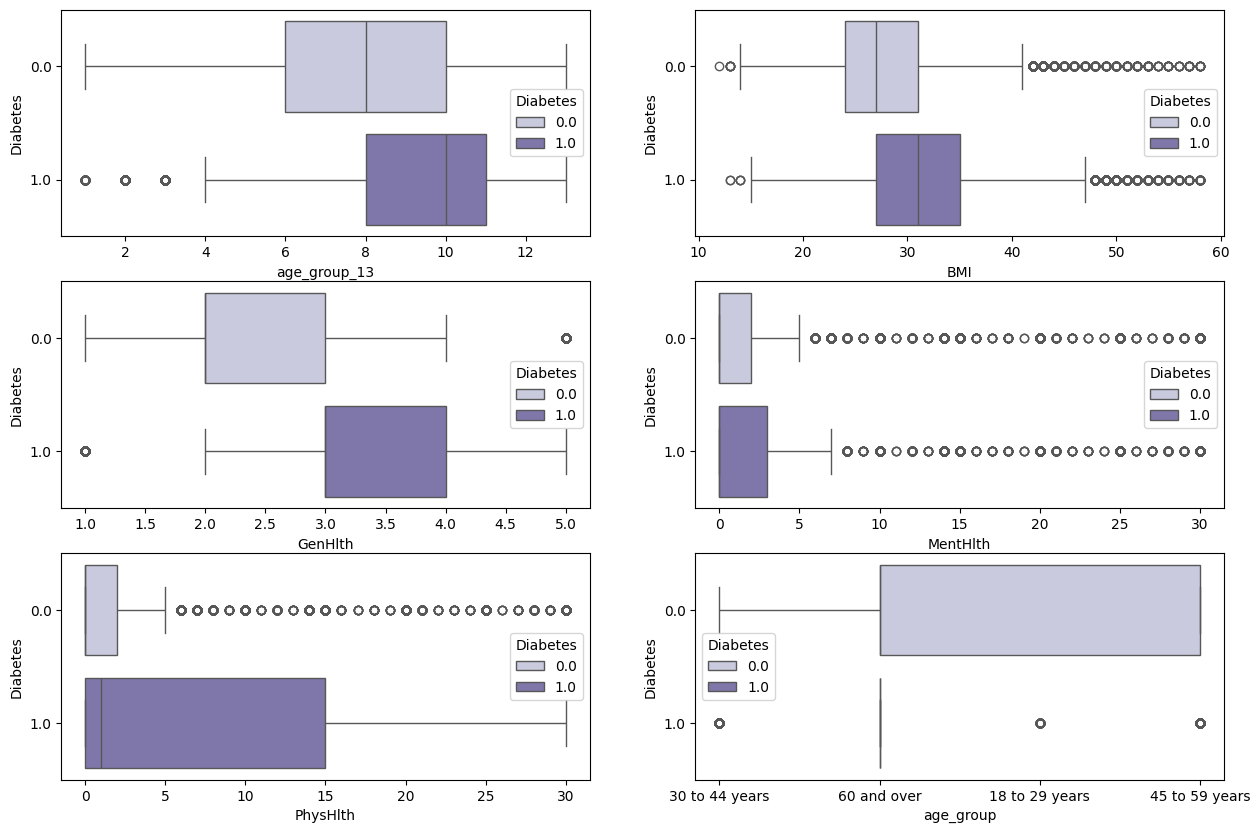
\includegraphics[width=1\linewidth]{raport/graphs/diabetes_boxplots.png}
    \caption{Enter Caption}
    \label{fig:enter-label}
\end{figure}

\begin{figure}
    \centering
    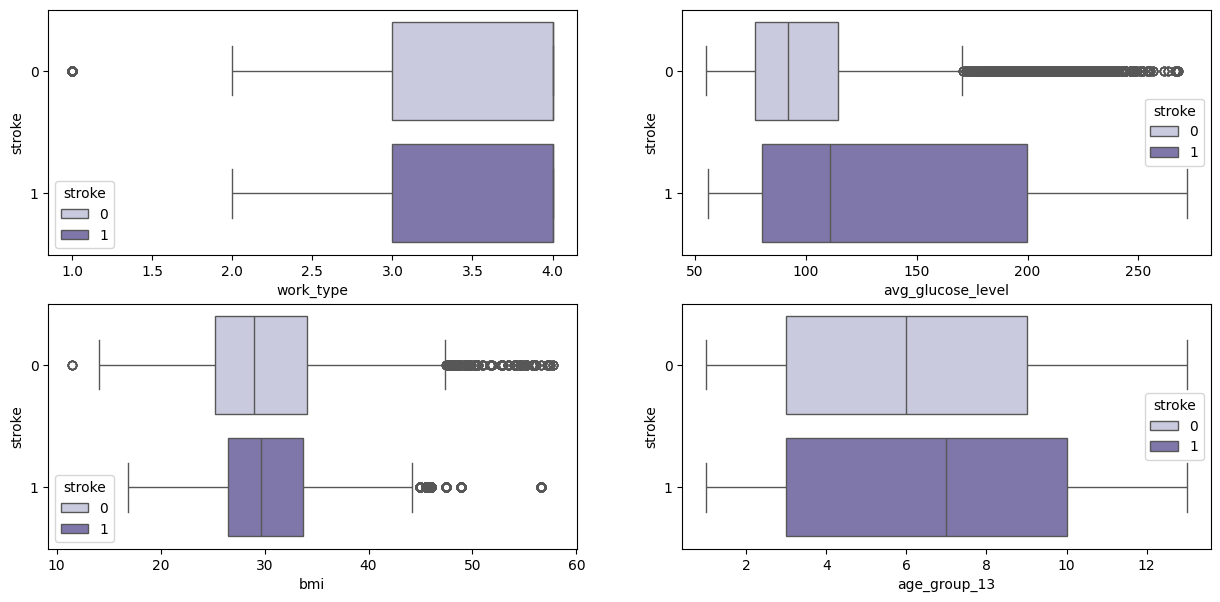
\includegraphics[width=1\linewidth]{raport/graphs/stroke_boxplots.png}
    \caption{Enter Caption}
    \label{fig:enter-label}
\end{figure}

\begin{figure}
    \centering
    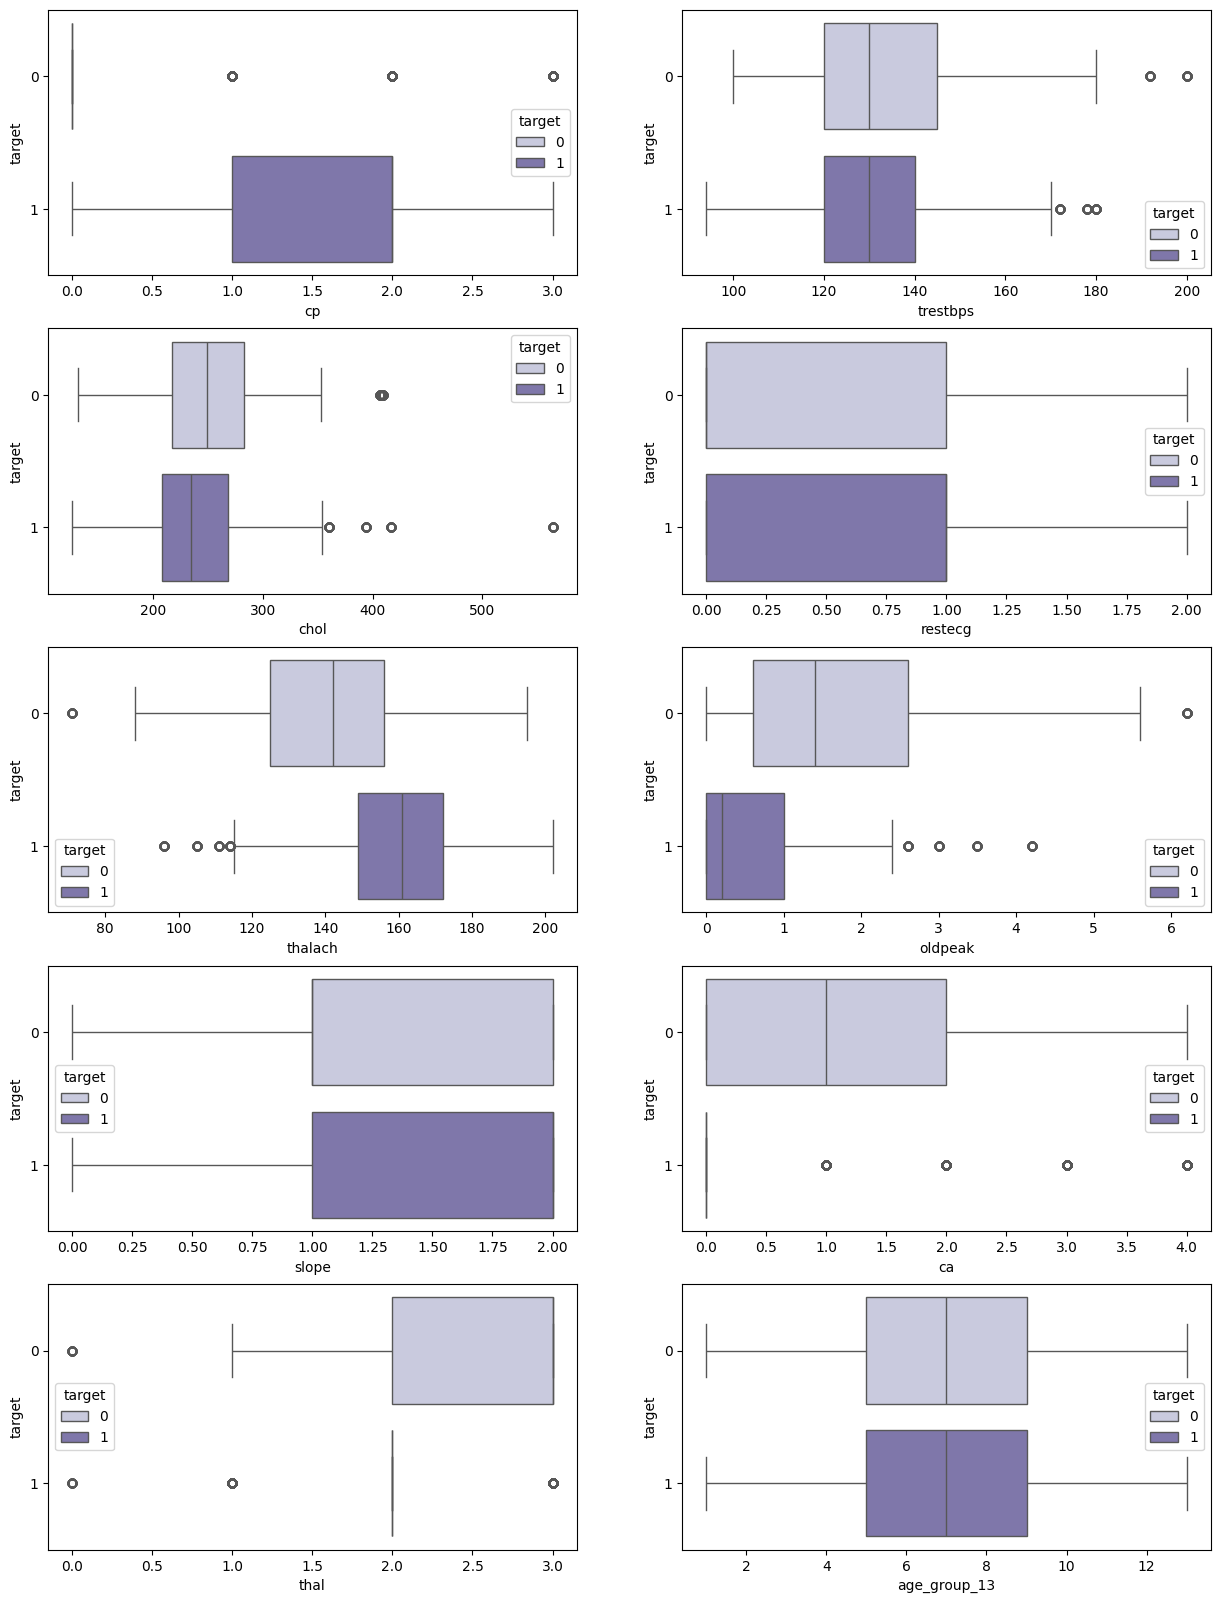
\includegraphics[width=1\linewidth]{raport/graphs/hypertension_boxplot.png}
    \caption{Enter Caption}
    \label{fig:enter-label}
\end{figure}

Rozkład BMI dla osób z cukrzycą wskazuje na wyższe wartości w porównaniu do osób bez cukrzycy, co sugeruje związek między wyższym BMI a zwiększonym ryzykiem cukrzycy. Ponadto osoby z cukrzycą częściej oceniają swój ogólny stan zdrowia (GenHlth), jak i zdrowie.

Natomiast osoby z nadciśnieniem mają niższe maksymalne tętno (thalach) w porównaniu z osobami bez nadciśnienia, co może odzwierciedlać wpływ choroby na kondycję serca.Zauważalne są wyższe wartości depresji ST (oldpeak) w EKG u osób z nadciśnieniem, co może wskazywać na związane z nim problemy sercowe.

Istotnie wyższe poziomy glukozy we krwi (avg glucose level) są obserwowane u osób, które doświadczyły udaru, co sugeruje silny związek między tym parametrem, a ryzykiem udaru. Podobnie osoby, które doświadczyły udaru, częściej znajdują się w kategoriach pracy bardziej stresujących lub mniej aktywnych fizycznie, co może przyczyniać się do zwiększonego ryzyka wystąpienia choroby.

W kolejny etapie przedstawiono macierze korelacji - narzędzie statystyczne używane do ilościowego określenia i wizualizacji siły i kierunku związku między zmiennymi w zbiorze danych. Każdy element macierzy przedstawia współczynnik korelacji między parami zmiennych, gdzie wartości bliskie +1 lub -1 wskazują na silną korelację dodatnią lub ujemną, a wartości bliskie zeru oznaczają brak zauważalnego związku.



\begin{figure}
    \centering
    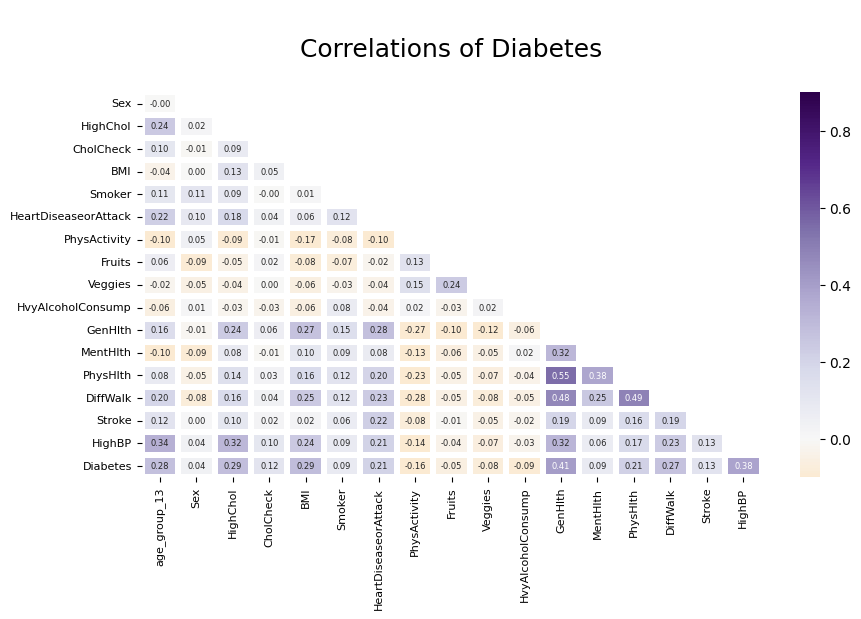
\includegraphics[width=0.9\linewidth]{raport/graphs/diabetes_corr.png}
    \caption{Enter Caption}
    \label{fig:enter-label}
\end{figure}

\begin{figure}
    \centering
    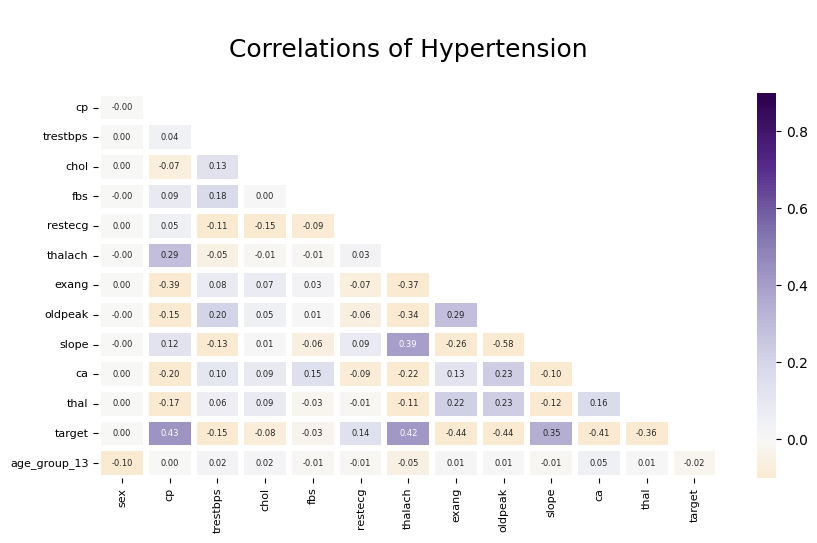
\includegraphics[width=0.9\linewidth]{raport/graphs/hypertension_corr.png}
    \caption{Enter Caption}
    \label{fig:enter-label}
\end{figure}

\begin{figure}
    \centering
    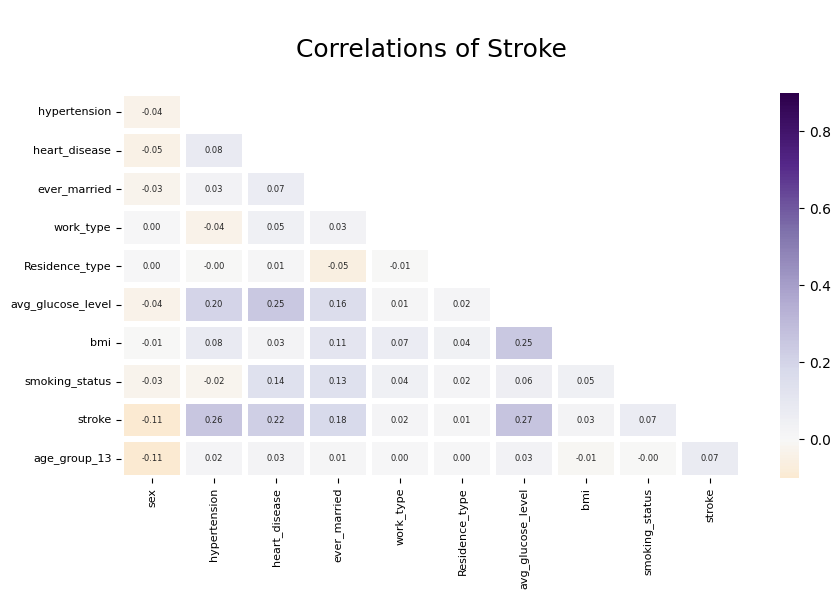
\includegraphics[width=0.9\linewidth]{raport/graphs/stroke_corr.png}
    \caption{Enter Caption}
    \label{fig:enter-label}
\end{figure}


histogramy czestosciowe (countplot) dla cech binarny z wyodrebnieniem istnienia danej choroby. konkretnie wskazuja czy dana cecha moze miec wplyw na chorobę.

\begin{figure}
    \centering
    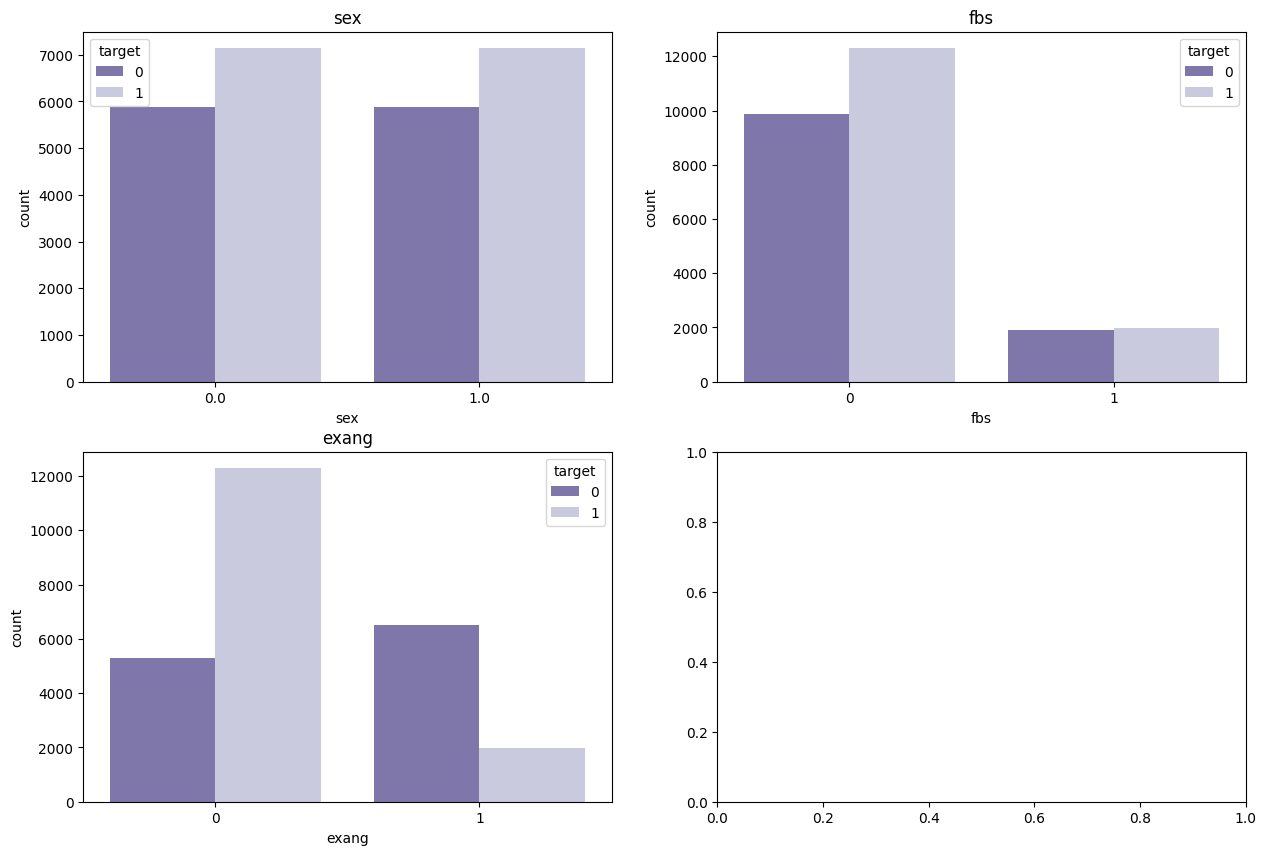
\includegraphics[width=0.9\linewidth]{raport/graphs/hypertension_binary.png}
    \caption{Enter Caption}
    \label{fig:enter-label}
\end{figure}

\begin{figure}
    \centering
    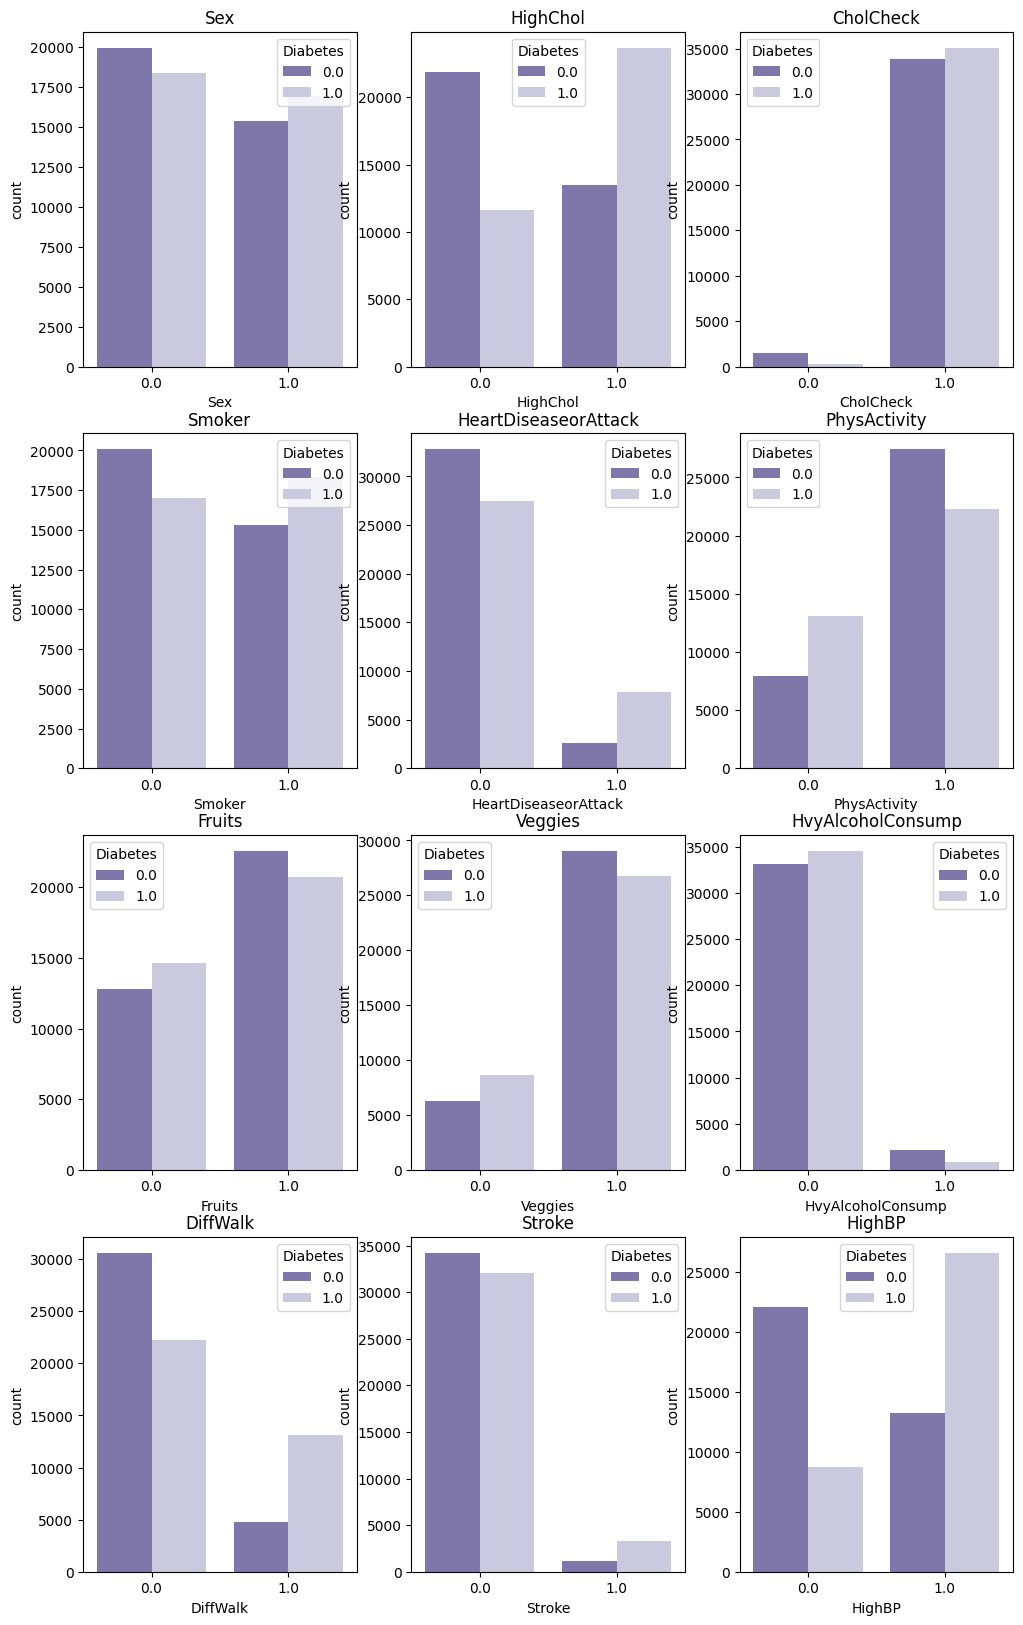
\includegraphics[width=1\linewidth]{raport/graphs/diabetes_binary.png}
    \caption{Enter Caption}
    \label{fig:enter-label}
\end{figure}

\begin{figure}
    \centering
    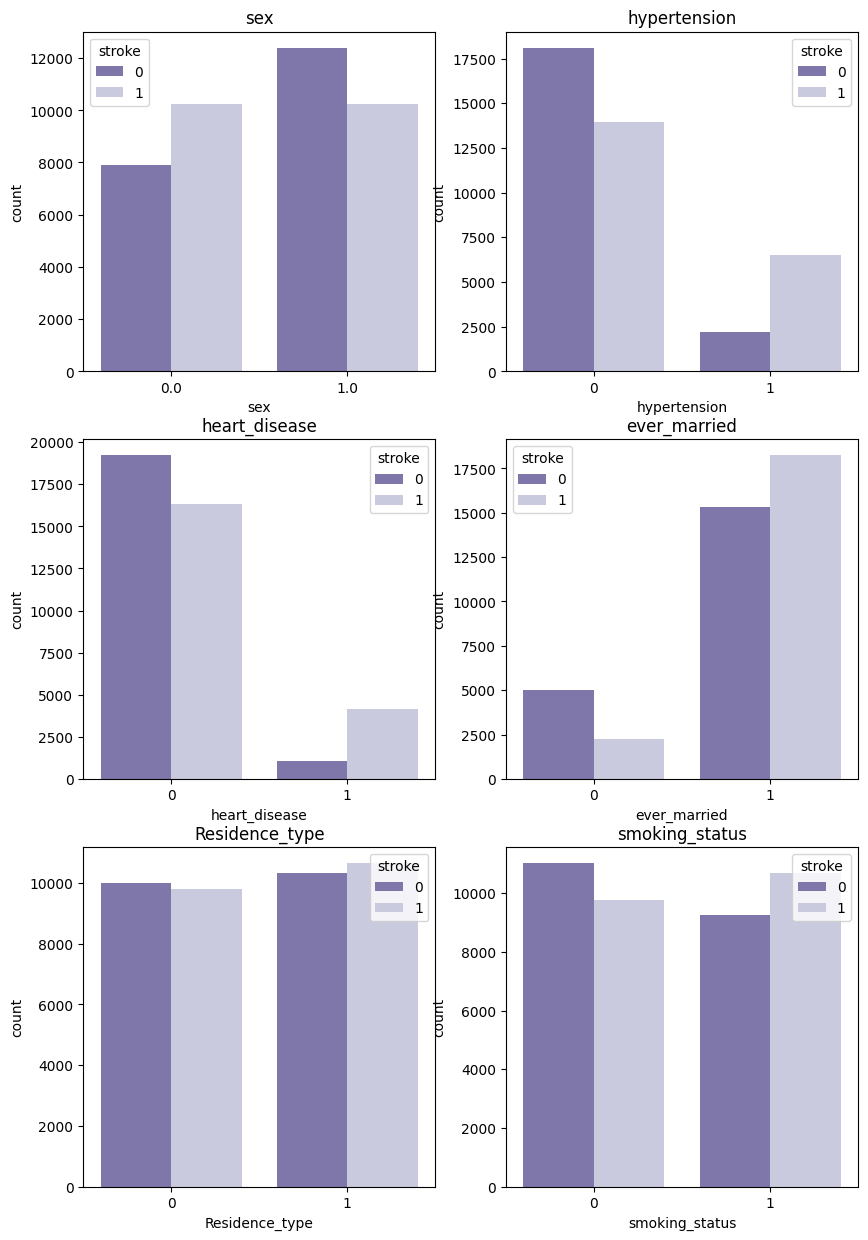
\includegraphics[width=1\linewidth]{raport/graphs/stroke_binary.png}
    \caption{Enter Caption}
    \label{fig:enter-label}
\end{figure}

\newpage
Czy wyszlo cos nieoczekiwanego?

PROFIL PACJENTA CUKRZYCA
- wysoki cholesterol
- palenie Have you smoked at least 100 cigarettes in your entire life? [Note: 5 packs = 100 cigarettes]
- choroby serca (coronary heart disease (CHD) or myocardial infarction (MI))
- brak aktywnosci physical activity in past 30 days
- dieta (malo warzywa i owoce)
- trudnosci w poruszaniu sie + udar
- nadcisnienie duuzy wplyw
- gorsze zdrowie mentalne i fizyczne + wyzsze bmi
- alkohol nie ma duzego znaczenia

PROFIL PACJENTA UDAR
- 
- 
- 
- 


PROFIL PACJENTA NADCISNIENIE
-
-
- 
- 


\newpage

\section{PCA}
\section{Predykcja wystąpienia choroby}
\subsection{Wybór modeli}
\subsection{Ocena jakości}
\section{Analiza czynników ryzyka/Podsumowanie}
udalo sie? 

\begin{thebibliography}{9}
\end{thebibliography}

\end{document}
